	\subsection{Abhören von verschlüsselter Kommuniktion bei bekannten Schlüsseln}
	% TODO@16.11.
	Als praktisches Beispiel wird eine Testumgebung mit folgender Hardware aufgebaut
	\begin{itemize}
		\item 1x Switch
		\item 2x PC
		\item 1x Webserver
	\end{itemize}
	Dabei wird die Hardware nach folgendem Schema eingerichtet. Ein PC dient dabei als "BadGuy", der als 3. Person versucht
	die Kommunikation zwischen den zwei anderen Teilnehmern (PC und Webserver) zu entschlüsseln.
	\begin{figure}[H]
		\centering
		%\includegraphics[width=.8\textwidth]{""}
		\caption{Darstellung Versuchsaufbau}
		\label{fig:versuchsaufbau}
	\end{figure}
	Der Switch wird mit unten aufgeführten Befehlen so eingerichtet, dass auf dem Interface Fa0/21 ein Switchport Analyzer (siehe Exkurs \ref{sec:exkurs_span}) eingesetzt wird.
	\commandbox{conf t}
	\commandbox{monitor session 1 source interface Fa0/1}
	\commandbox{monitor session 1 destination interface Fa0/21 encapsulation repliate}
	
	Der Versuch besteht aus 2 Teilversuchen. Im ersten Teilversuch wurde auf dem SPAN Port angeschlossenen Rechner das Programm Wireshark gestartet ohne dabei die SSL Zertifikate auszutauschen. Das Ergebnis, ein gesnifftes TCP Paket auf dem 443 Port ist im Bild \ref{fig:ssl_encrypted_data} zu sehen.
	\begin{figure}[H]
		\centering
		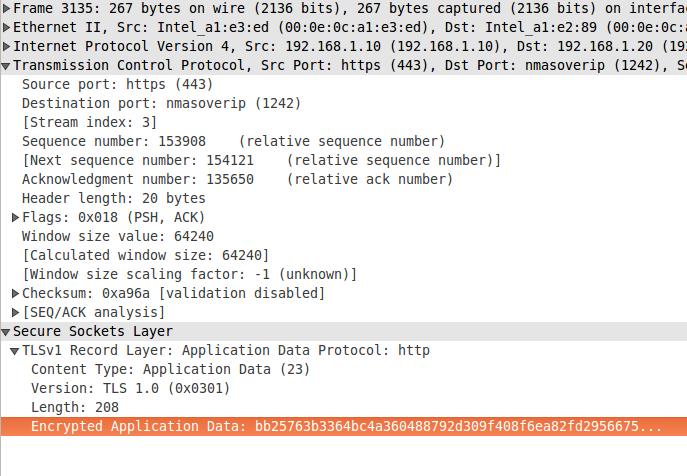
\includegraphics[width=.8\textwidth]{SSL_encrypted_data.png}
		\caption{Ansicht eines TCP Pakets mit SSL Verschlüsselung}
		\label{fig:ssl_encrypted_data}
	\end{figure}
	
	Beim zweiten Teilversuch wurde dem Wireshark der Schlüssel mitgeteilt. Über Settings unter Protokolle im Tab SSL wurde das Zertifikat "<hier cert name>" dem Wireshark SSL Protkoll zur Verfügung gestellt (siehe Bild \ref{fig:ssl_settings}).
	\begin{figure}[H]
		\centering
		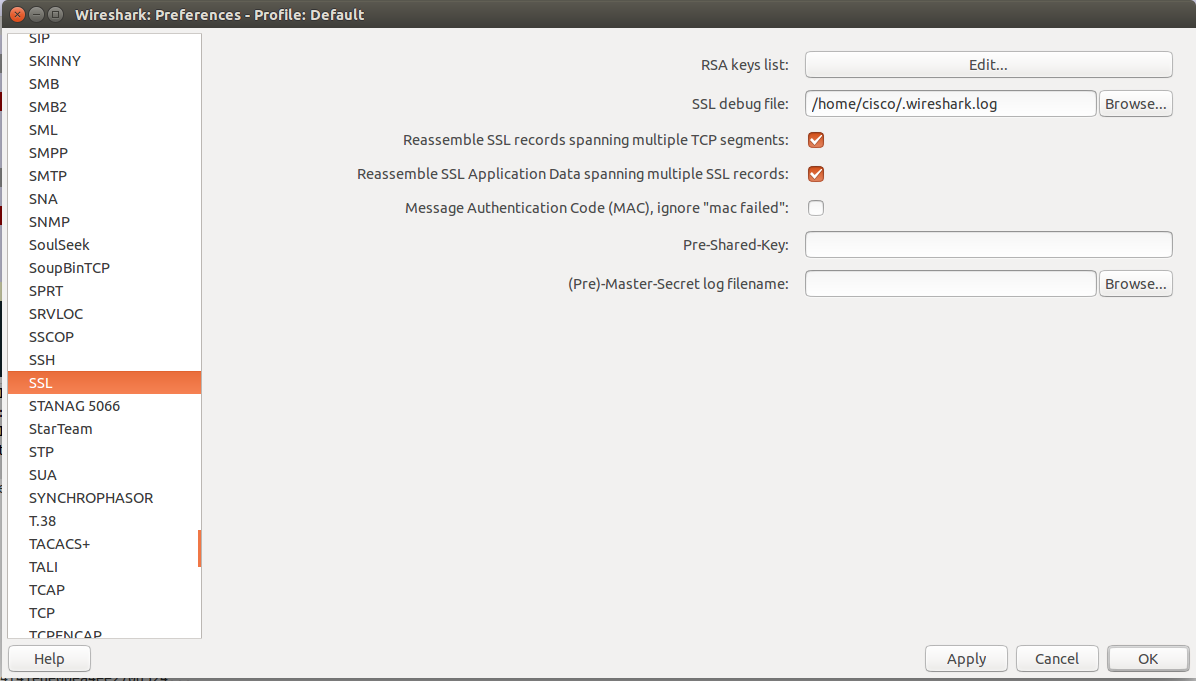
\includegraphics[width=.8\textwidth]{SSL_settings.png}
		\caption{Einstellungen für die SSL Key Übergabe}
		\label{fig:ssl_settings}
	\end{figure}
	Durch den Versuch wurde die Nachricht leider nicht lesbar entschlüsselt. Nach \citeA{wireshark} auf der Wireshark Website kann das Programm nur Schlüssel verwenden, welche nicht durch ein Passwort verschlüsselt sind. Das wurde durch ein umformen des Keys gelöst. Danach trat ein weiteres Problem ... %@TODO finish fazit des versuchs
	\shadebox{
		\subsection*{Exkurs: Switch Port Analyzer (SPAN)}\label{sec:exkurs_span}
		Switch Port Analyzer (kurz SPAN), oft auch port mirroring oder port monitoring genannt, kopiert switch netzwerk verkehr und sendet diesen an den SPAN Port zur Analyse durch einen Netzwerk Analyzer weiter. Durch Einschalten des SPAN, kann der Verkehr auf einem Switch überwacht werden durch Weiterleiten von eingehendem und ausgehendem Nachrichten an einen anderen Port [...] Netzwerk Analyzer können so zum Fehlersuchen von Netzwerkproblemen im Datenverkehr benutzt werden, ohne dass dabei das Netzwerk ausser Dienst genommen werden muss.\cite{span}
		}
		
	\subsection{Analyse von bereits vorhandenen Tools} % keine Enterprise-lösungen
	%Daniel